\documentclass[10pt]{article}

%-------------PACKAGES------------- 
\usepackage[margin=1in]{geometry} 
\usepackage{amsmath,amsthm,amssymb}
\usepackage{pgfplots}
\usepackage{float}
\usepackage{braket}
\usepackage{titling}
\usepackage{tikz}
\usepackage{mathtools}
\usepackage{listings}
\usepackage{color}
\usepackage{caption}
\usepackage{subcaption}

%-------------FORMATTING-------------
\setlength{\droptitle}{-5em} 
\setlength{\parindent}{0pt}
 
%--------------COMMANDS--------------
\newcommand{\N}{\mathbb{N}}
\newcommand{\Z}{\mathbb{Z}}
\newcommand{\R}{\mathbb{R}}
\newcommand{\C}{\mathbb{C}}
%\renewcommand{\qedsymbol}{\filledbox}
\newcommand\numberthis{\addtocounter{equation}{1}\tag{\theequation}}

\DeclarePairedDelimiter \abs{\lvert}{\rvert}%
\DeclarePairedDelimiter \norm{\lVert}{\rVert}%

%------------ENVIRONMENTS------------ 
\newenvironment{theorem}[2][]{\begin{trivlist}
\item[{\bfseries #1}\hskip \labelsep {\bfseries #2.}]}{\end{trivlist}}
\newenvironment{lemma}[2][Lemma]{\begin{trivlist}
\item[\hskip \labelsep {\bfseries #1}\hskip \labelsep {\bfseries #2.}]}{\end{trivlist}}
\newenvironment{exercise}[2][Exercise]{\begin{trivlist}
\item[\hskip \labelsep {\bfseries #1}\hskip \labelsep {\bfseries #2.}]}{\end{trivlist}}
\newenvironment{reflection}[2][Reflection]{\begin{trivlist}
\item[\hskip \labelsep {\bfseries #1}\hskip \labelsep {\bfseries #2.}]}{\end{trivlist}}
\newenvironment{proposition}[2][Proposition]{\begin{trivlist}
\item[\hskip \labelsep {\bfseries #1}\hskip \labelsep {\bfseries #2.}]}{\end{trivlist}}
\newenvironment{corollary}[2][Corollary]{\begin{trivlist}
\item[\hskip \labelsep {\bfseries #1}\hskip \labelsep {\bfseries #2.}]}{\end{trivlist}}
\theoremstyle{remark}
\newtheorem*{remark}{Remark}

%------------------------------------ 
%---------START-OF-DOCUMENT----------
%------------------------------------
\begin{document}
 
\title{Homework 4}
\author{David Miller \\ 
MAP 5345: Partial Differential Equations I} 
 
\maketitle

\subsection*{Problem 1}

\textit{Consider heat conduction in a rod with insulating ends, so that we have vanishing Neumann boundary conditions}
\begin{align}
	& u_t = ku_{xx} \quad \text{ for } 0 < x < L, t > 0 \\
	& u_x(0,t) = u_x(L,t) = 0 \\
	& u(x,0) = u_0(x)
\end{align}

\textit{(a) Use separation of variables to find the general solution (as done in class).} \\ 

Assume $u(x,t)$ has a solution in the form of a product
\begin{align*}
	& u(x,t) = X(x)T(t)
\end{align*}

Plugging this back into (1) we get
\begin{align*}
	X(x)\frac{dT(t)}{dt} = kT(t)\frac{d^2 X(x)}{dx^2}
\end{align*}

However, the only way a function of $x$ can equal a function of $t$ is if they both equal some constant $\lambda$:
\begin{align*}
	\frac{1}{k}\frac{dT(t)}{dt} = \frac{d^2X(x)}{dx^2} = -\lambda
\end{align*}

Solving the differential equations we are left with
\begin{align*}
	T(t) & = e^{-k\lambda t} \\
	X(x) & = a cos(\sqrt{\lambda}x) + bcos(\sqrt{\lambda} x), \quad a,b \in \mathbb{R}
\end{align*}

Applying the Neumann boundary conditions we get
\begin{align*}
	X^\prime(x) & = -asin(\sqrt{\lambda} x) + bcos(\sqrt{\lambda} x) \\
	X^\prime(0) & = b = 0 \\
	X^\prime(L) & = -asin(\sqrt{\lambda} x) = 0 \Rightarrow \lambda_n  = n^2\pi^2/L^2
\end{align*}

Using our eigenvalue and eigenfunctions $T_n(t)$ and $X_n(x)$ we apply the Principle of Superposition to derive a general solution
\begin{align*}
	& u(x,t) = \sum\limits_{n=0}^\infty a_nT_n(t)X_n(x) \\
	\Rightarrow & \, \boxed{u(x,t) = a_0 + \sum\limits_{n=1}^\infty a_ncos(n\pi x/L)e^{-k\frac{n^2\pi^2}{L^2}}t} \numberthis
\end{align*}

Now we need to determine the coefficients $a_n$. To do this let us quickly reabsorb $a_0$ back into the sum then take the inner product of both sides of $(\star)$ w.r.t. $X_m(x)$ evaluated at $t = 0$:
\begin{align*}
\int\limits_0^L u_0(x)cos(m\pi x/L) \, dx = \sum\limits_{n=0}^\infty\int\limits_0^L a_ncos(n\pi x/L)cos(m\pi x/L) \, dx, \quad m = 1,2,\ldots \tag{$\star$}
\end{align*}

To evaluate $\braket{X_n,X_m}$ we convert $X_n$ and $X_m$ into exponentials
\begin{align*}
	\braket{X_n, X_m} & = \int\limits_0^L cos(n\pi x/L)cos(m\pi x/L) \ dx \\
	& = \int\limits_0^L \frac{e^{in\pi x/L} + e^{-in\pi x/L}}{2}\frac{e^{im\pi x/L} + e^{-im\pi x/L}}{2} \, dx \\
	& = \frac{1}{4} \int\limits_0^L e^{i(n+m)\pi x/L} + e^{i(n-m)\pi x/L} + e^{-i(n-m)\pi x/L} + e^{-i(n+m)\pi x/L} \, dx \\
	& = \frac{1}{2}\int\limits_0^L cos((n+m)\pi x/L) + cos((n-m)\pi x/L) \, dx \\
	& = {
	\begin{cases}
	\bigg(\frac{L}{2(n+m)\pi}sin((n+m)\pi x/L) + \frac{L}{2(n-m)\pi}sin((n-m)\pi x/L)\bigg)\bigg\vert_0^L & n \neq m \\
	\bigg(\frac{x}{2} + \frac{L}{2(n+m)\pi}sin((n+m)\pi x/L)\bigg)\bigg\vert_0^L & n = m
	\end{cases}} \\
	& = \delta_{nm}\frac{L}{2}
\end{align*}

where $\delta_{ij}= 1$ if $i = j$ and 0 otherwise. Plugging this back into $(\star)$ we get 
\begin{align}
	\boxed{a_n = \frac{\braket{u_0, X_n}}{\braket{X_n, X_n}} = \frac{2}{L(1 + \delta_{0n})}\int\limits_0^L u_0(x)cos(n\pi x/ L) \, dx, \quad n = 0,1,\ldots}
\end{align}

\textit{(b) Prove that the eigenfunctions $X_n(x) = cos(n\pi x/L)$ are orthogonal with respect to the 'inner product' $\Braket{f,g} = \int_0^L f(x)g(x)dx$.} \

\begin{proof}
From part (a) we have that $\braket{X_n,X_m} = \delta_{nm}\frac{L}{2}$ over the domain $[0,L]$. This shows that the eigenfunctions $X_n = cos(n\pi x/L)$ are orthogonal.
\end{proof}

\textit{(c) Consider the initial condition $u_0 = x(L-x)$. Use projection to determine the coefficients in the general solution and thus obtain the solution to the IBVP. Pay attention to the decay rate of the coefficients.} \\ 

Using (5) and substituting $x(L-x)$ for $u_0(x)$ we get
\begin{align*}
	a_n & = \frac{2}{L(1 + \delta_{0n})}\int\limits_0^L x(L-x)cos(n\pi x/L) \, dx \\
	& = \frac{2}{L(1 + \delta_{0n})}\bigg(\underbrace{x(L-x)\frac{L}{n\pi}sin(n\pi x/L)\bigg\vert_0^L}_{= 0 \text{ by boundary conditions}} - \frac{L}{n\pi}\int\limits_0^L (L - 2x)sin(n\pi x/L) \, dx\bigg) \\ 
	& = \frac{-2}{n\pi(1 + \delta_{0n})}\bigg(-\frac{L}{n\pi}(L - 2x)cos(n\pi x/L)\bigg\vert_0^L - \frac{2L}{n\pi}\int\limits_0^L cos(n\pi x/L) \, dx\bigg) \\
	& = \frac{-2L^2}{n^2\pi^2(1 + \delta_{0n})}\bigg(-Lcos(n\pi) - L\bigg) \\
	& = {
		\begin{cases}
		\frac{-4L^2}{n^2\pi^2(1 + \delta_{0n})} & n \text{ even} \\
		0 & n \text{ odd}
		\end{cases}
		}
\end{align*}

However we can not use this to evaluate the case $n = 0$ so we take a step back to evaluate $a_0$:
\begin{align*}
	a_0 & = \frac{1}{L}\int\limits_0^L x(L-x)cos(0) \, dx \\
	& = \bigg(\frac{x^2}{2} - \frac{x^3}{3L}\bigg)\bigg\vert_0^L = \frac{L^2}{6}
\end{align*}

Putting all this together we get that 
\begin{align*}
	\boxed{a_0 = \frac{L^2}{6}, \quad a_{2n} = \frac{-4L^2}{n^2\pi^2} \text{ for } n = 1,2,\ldots}
\end{align*}

\textit{(d) Set $k = 0.5$ and $L = 1$. Use Julia to plot the solution at a few times. Notice that the initial condition does not satisfy the boundary right conditions, but that turns out to be okay. Somehow the solution automatically adjusts to satisfy the boundary conditions a short time after $t = 0$. From your graphs, see if you can estimate the earliest time at which the boundary conditions are satisfied. Can you prove a result?} \\

Below is a figure of our IBVP evolving from $t = 0$ to $t = 1$. As we can see the heat collapses to a uniform distribution. This is expected of Neumann boundary conditions since it's physical interpretation is insulated ends. In fact as $t \rightarrow \infty$ the sum in $(4) \rightarrow 0$ so the solution $u(x,t) \rightarrow a_0$. This is the uniform distribution that Neumann boundary conditions guarantees. From inspection we can see that it does indeed go to $L^2/6 \approx 0.167$.

\begin{figure}[H]
	\centering
	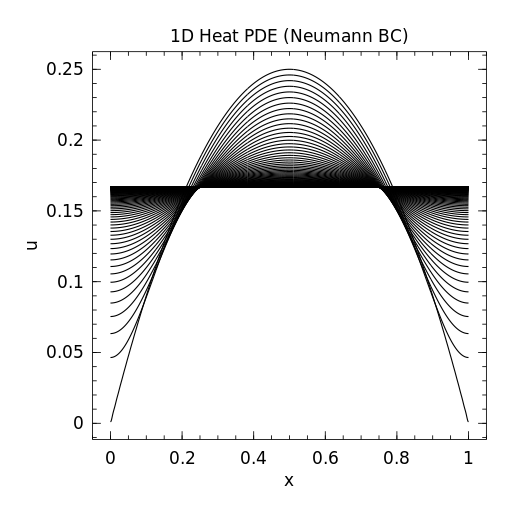
\includegraphics[width = 10cm]{1d_1.png}
	\caption{Solution to IBVP with $\Delta t = 1/250$, $\Delta x = 1/1000$, and truncation value $N  = 100$.}
\end{figure} 

We can see in Figure 1 that our solution satisfies our initial parabolic heat distribution and then collapses to uniform heat distribution as we expect. However at $t = 0$ it does not seem to satisfy our Neumann boundary conditions (zero derivative at $x = 0$ and $x = L$). If we look at the boundaries at just $t = 1/10000$ we see that the boundary conditions seem to be satisfied.

\begin{figure}[H]
	\centering
	\begin{subfigure}{.5\textwidth}
		\centering
		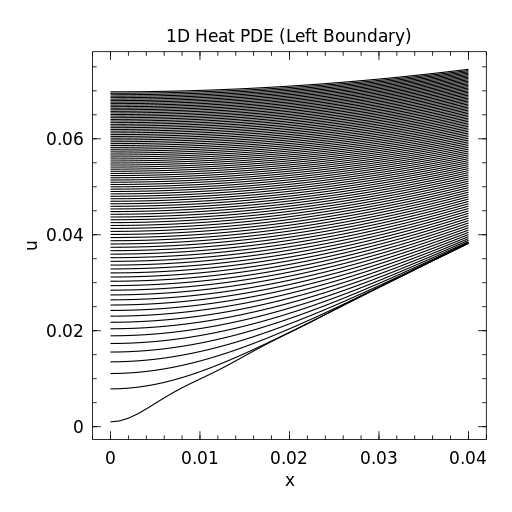
\includegraphics[width=0.8\linewidth]{1d_2.png}
		\caption{$\Delta x = 1/1000$ and $\Delta t = 1/10000$.}
		\label{fig:sub1}
	\end{subfigure}%
	\begin{subfigure}{.5\textwidth}
		\centering
		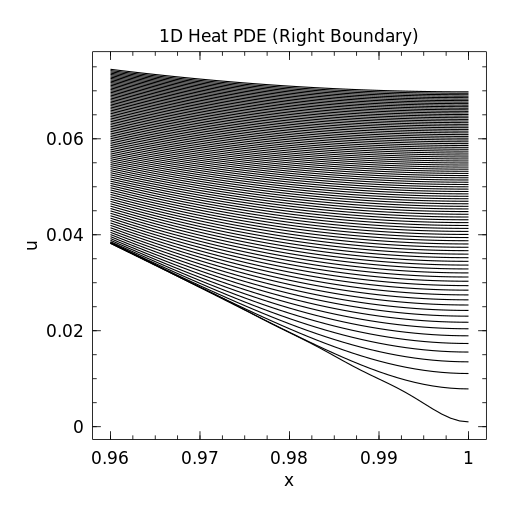
\includegraphics[width=0.8\linewidth]{1d_3.png}
		\caption{$\Delta x = 1/1000$ and $\Delta t = 1/10000$.}
		\label{fig:sub2}
	\end{subfigure}
	\caption{The left and right boundaries show that the Neumann condition is satisfied any time $t > 0$.}
	\label{fig:test}
\end{figure}  

\newpage

\subsection*{Problem 2}

\textit{Consider the wave equation with vanishing Dirichlet boundary conditions}
\begin{align}
	& u_{tt} = c^2u_{xx} \\
	& u(0,t) = u(L,t) = 0	 
\end{align}

\textit{Define the 'energy' as}
\begin{align}
	& E = \frac{1}{2}\int\limits_{0}^{L} u_{t}^2 + c^2u_x^2 \, dx
\end{align}

\textit{Prove that the energy is conserved.} 

\begin{proof}
Taking the time derivative $\partial_t$ of (6) we get
\begin{align*}
	\partial_t E & = \partial_t \bigg( \frac{1}{2}\int\limits_0^L u_t^2 + c^2 u_x^2 \, dx \bigg) \\
	& = \int\limits_0^L u_t u_{tt} + c^2 u_x u_{xt} \, dx. \tag{$\star$}
\end{align*} 

Setting $w = u_x$, ${dw} = u_{xx} \, dx$, ${dv} = u_{xt} \, dx$ and $v = u_x$ we get that the latter part of $(\star)$ is
\begin{align*}
	\int\limits_0^L c^2u_xu_{xt} \,dx = \int\limits_0^L w \, dv & = wv\bigg\vert_0^L - \int\limits_0^L v \, dw \\
	& = c^2u_tu_x\bigg\vert_0^L - c^2\int\limits_0^L u_tu_{xx} \, dx. 
\end{align*}

Plugging this back into $(\star)$ we get
\begin{align*}
	& \int\limits_0^L u_t u_{tt} \, dx - \int\limits_0^L c^2u_tu_{xx} \, dx + c^2u_xu_t\bigg\vert_0^L \\
	= & \int\limits_0^L u_t\underbrace{\bigg( u_{tt} - c^2u_{xx} \bigg)}_{= 0 \text{ by wave equation}} \, dx + c^2u_xu_t\bigg\vert_0^L
\end{align*}

Now we are just left with evaluating $c^2u_xu_t$ at the boundaries ($x = 0$ and $x = L$). However, since we have Dirichlet boundary conditions we know that the ends are clamped so they do not change their position. We can then set $u_t$ = 0 at the boundaries which effectively makes the remaining term zero. Therefore 'energy' is conserved.
\end{proof}

\newpage

\subsection*{Problem 3}

\textit{Consider the real and complex representation of Fourier series}
\begin{align}
	& f(x) = \frac{1}{2}a_0 + \sum\limits_{n=1}^\infty a_n cos(n\pi x/L) + b_n sin(n\pi x/L) \\
	& f(x) = \sum\limits_{n = -\infty}^\infty c_n e^{in\pi x/L}
\end{align}

\textit{where $a_n, b_n \in \mathbb{R}$ and $c_n \in \mathbb{C}$.} \\ \\
\textit{(a) Derive formulas to calculate the complex coefficients $c_n$ in terms of $a_n$ and $b_n$, and vice versa. This gives us an easy way to transform between the real and complex representations.} \\

Using Euler's Formula we can write $cos(x)$ and $sin(x)$ in terms of $e^{i\pi x}$: 
\begin{align*}
	& cos(x) = \frac{e^{i \pi x} + e^{-i\pi x}}{2} \quad\quad\quad sin(x) = \frac{e^{i\pi x} - e^{-i\pi x}}{2i}. \tag{$\star$}
\end{align*}

Using $(\star)$ we can convert (9) $\rightarrow$ (10) to determine $c_n$ in terms of $a_n$ and $b_n$:
\begin{align*}
	f(x) & = \frac{1}{2}a_0 + \sum\limits_{n=1}^\infty a_n cos(n\pi x/L) + b_n sin(n\pi x/L) \\
	& = \frac{1}{2}a_0 + \sum\limits_{n=1}^\infty a_n\frac{e^{in\pi x/L} + e^{-in\pi x/L}}{2} + b_n\frac{e^{in\pi x/L} - e^{-in\pi x/L}}{2i} \\
	& = \frac{1}{2}a_0 + \sum\limits_{n=1}^\infty \bigg(\frac{a_n}{2} + \frac{b_n}{2i}\bigg)e^{in\pi x/L} + \bigg(
	\frac{a_n}{2} - \frac{b_n}{2i}\bigg)e^{-in\pi x/L} \\
	& = \frac{1}{2}a_0 + \sum\limits_{n=-\infty}^{-1}\frac{a_{-n} + ib_{-n}}{2}e^{in\pi x/L} + \sum\limits_{n=1}^\infty \frac{a_n - ib_n}{2}e^{in\pi x/L} \tag{using $\frac{b_n}{2i} = \frac{-ib_n}{2}$} \\
	\Rightarrow & \boxed{c_{-n} = c_{\abs{n}}^\star = \frac{a_{n} + ib_{n}}{2} \text{ for } n = \ldots,-2,-1 \quad c_n = \frac{a_n - ib_n}{2} \text{ for } n = 1,2,\ldots} \numberthis
\end{align*}

where $c^\star$ is complex conjugate. To convert (10) $\rightarrow$ (9) and determine $a_n$ and $b_n$ in terms of $c_n$ we use Euler's formula and the fact $cos(-x) = cos(x)$ and $sin(-x) = -sin(x)$ to rewrite (10) as a sum from $n = 1$ to $\infty$:
\begin{align*}
	& \sum\limits_\infty^\infty c_n e^{in\pi x/L} = \sum\limits_{n=1}^\infty c_{-n}\bigg(cos(n\pi x/L) - isin(n\pi x/L)\bigg) + c_n\bigg(cos(n\pi x/L + isin(n\pi x/L)\bigg)
\end{align*}

We can then set this equal to (9) to determine $a_n$ and $b_n$:
\begin{align*}
 \sum\limits_{n=1}^\infty c_{-n}\bigg(cos(n\pi x/L) - isin(n\pi x/L)\bigg) + c_n\bigg(cos(n\pi x/L + isin(n\pi x/L)\bigg) = \sum\limits_{n=1}^\infty a_n cos(n\pi x/L) + b_n sin(n\pi x/L) 
\end{align*}

Since the sums are over the same index we can equate the insides of both:
\begin{align*}
	 (c_n + c_{-n})&cos(n\pi x/L) + i(c_n - c_{-n})sin(n\pi x/L) = a_ncos(n\pi x/L) b_nsin(n\pi x/L) \\
	 \Rightarrow & \, \boxed{a_n = c_n + c_{-n} = 2\mathcal{R}(c_n), \quad b_n = i(c_n - c_{-n}) = 2\mathcal{I}(c_n)} \numberthis
\end{align*}

where $\mathcal{R}$ is the real part and $\mathcal{I}$ is the imaginary part.

\newpage

\textit{(b) If $f(x)$ is real valued, what relationship between $c_n$ and $c_{-n}$ must be satisfied?}

\begin{proposition}{1}
If $f(x)$ is a real valued function for all $x$ then $c_n$ and $c_{-n}$ must be complex conjugates.
\end{proposition}

\begin{proof}
This proof will rely on geometric interpretation of complex numbers. The complex Fourier series can be represented as
\begin{align*}
f(x) & = \sum\limits_{n=1}^\infty c_{-n}\bigg(cos(n\pi x/L) - isin(n\pi x/L)\bigg) + c_n\bigg(cos(n\pi x/L + isin(n\pi x/L)\bigg) \\
& = \sum\limits_{n=1}^\infty c_{-n}e^{-im\pi x/L} + c_me^{im\pi x/L}
\end{align*}	
It is enough to prove $c_{-m}e^{-im\pi x/L} + c_me^{im\pi x/L}$ is real valued for any arbitrary integer $m$. The $e^{im\pi x/L}$ term is just a point on the unit circle in $\mathbb{C}$ with $\theta = m\pi x/L$ and $e^{-im\pi x/L}$ is its reflection about the $x$-axis. The coefficients $c_{-m}$ and $c_m$ scale their respective point by the same factor but $c_{-m}$ rotates the point $e^{-im\pi x/L}$ clockwise by $\theta$ while $c_m$ rotates $e^{im\pi x/L}$ counter-clockwise by $\theta$. 
\begin{center}
	\begin{tikzpicture}[baseline=(current bounding box.center)]
	\begin{axis}[
	trig format plots=rad,
	axis equal,
	hide axis
	]
	\node at (axis cs:-2,1.25) [anchor=south] {\Large$\mathbb{C}$};
	\node at (axis cs:1.25,.717) [anchor=south] {$e^{im\pi x/L}$};
	\node at (axis cs:1.25,-.717) [anchor=north] {$e^{-im\pi x/L}$};
	\addplot [only marks] table {
		 .707 .707
		 .707 -.707
	};
	\addplot [domain = 0:2*pi, samples=100, black, dashed] ({cos(x)}, {sin(x)});
	\addplot [domain = -1.5:1.5, samples=100, black] ({x}, {0});
	\addplot [domain = -1.5:1.5, samples=100, black] ({0}, {x});
	\addplot [domain = 0:1, samples=100, black] ({x/sqrt(2)}, {x/sqrt(2)});
	\addplot [domain = 0:1, samples=100, black] ({x/sqrt(2)}, {-x/sqrt(2)});
	\end{axis}
	\end{tikzpicture}$\xrightarrow{\text{apply }c_{-m} \text{ and } c_m}$
	\begin{tikzpicture}[baseline=(current bounding box.center)]
	\begin{axis}[
	trig format plots=rad,
	axis equal,
	hide axis
	]
	\node at (axis cs:-2,1.25) [anchor=south] {\Large$\mathbb{C}$};
	\node at (axis cs:1.25,.717) [anchor=south] {$e^{im\pi x/L}$};
	\node at (axis cs:1.25,-.717) [anchor=north] {$e^{-im\pi x/L}$};
	\node at (axis cs:-0.8,-1.25) [anchor=north] {$c_{-m}\star e^{-im\pi x/L}$};
	\node at (axis cs:-0.8,1.25) [anchor=south] {$c_{m}\star e^{-im\pi x/L}$};
	\addplot [only marks] table {
		.707 .707
		.707 -.707
		-0.75 1.25
		-0.75 -1.25
	};
	\addplot [domain = 0:2*pi, samples=100, black, dashed] ({cos(x)}, {sin(x)});
	\addplot [domain = -1.5:1.5, samples=100, black] ({x}, {0});
	\addplot [domain = -1.5:1.5, samples=100, black] ({0}, {x});
	\addplot [domain = 0:1, samples=100, black] ({x/sqrt(2)}, {x/sqrt(2)});
	\addplot [domain = 0:1, samples=100, black] ({x/sqrt(2)}, {-x/sqrt(2)});
	\addplot [domain = 0:0.75, samples=100, black] ({-x}, {-5*x/3});
	\addplot [domain = 0:0.75, samples=100, black] ({-x}, {5*x/3});
	\end{axis}
	\end{tikzpicture}
\end{center}

All that is left to do is sum $c_{-n}e^{-im\pi x/L}$ and $c_ne^{im\pi x/L}$. It is easy to see that their sum will be on the real line and therefore real valued. 

\begin{center}
\begin{tikzpicture}[scale = 1.25]
	\begin{axis}[
	trig format plots=rad,
	axis equal,
	hide axis
	]
	\node at (axis cs:-2,1.25) [anchor=south] {\Large$\mathbb{C}$};
	\node at (axis cs:1.25,.717) [anchor=south] {$e^{im\pi x/L}$};
	\node at (axis cs:1.25,-.717) [anchor=north] {$e^{-im\pi x/L}$};
	\node at (axis cs:-0.8,-1.25) [anchor=north] {$c_{-m}\star e^{-im\pi x/L}$};
	\node at (axis cs:-0.8,1.25) [anchor=south] {$c_{m}\star e^{-im\pi x/L}$};
	\node at (axis cs:-0.5,0) [anchor=south east] {$\vec{A}$};
	\addplot [only marks] table {
		.707 .707
		.707 -.707
		-0.75 1.25
		-0.75 -1.25
		-1.5 0
	};
	\addplot [domain = 0:2*pi, samples=100, black, dashed] ({cos(x)}, {sin(x)});
	\addplot [domain = -1.5:1.5, samples=100, black] ({x}, {0});
	\addplot [domain = -1.5:1.5, samples=100, black] ({0}, {x});
	\addplot [domain = 0:1, samples=100, black] ({x/sqrt(2)}, {x/sqrt(2)});
	\addplot [domain = 0:1, samples=100, black] ({x/sqrt(2)}, {-x/sqrt(2)});
	\addplot [domain = 0:0.75, samples=100, black] ({-x}, {-5*x/3});
	\addplot [domain = 0:0.75, samples=100, black] ({-x}, {5*x/3});
		\addplot [domain = 0:0.75, samples=100, black, dashed] ({-x-0.75}, {5*x/3 - 3.75/3});
		\addplot [domain = 0:0.75, samples=100, black, dashed] ({-x-0.75}, {-5*x/3 + 3.75/3});
		\addplot [domain = 0.65:0.75, samples=100, black, style = ultra thick] ({-x-0.75}, {5*x/3 - 3.75/3});
		\addplot [domain = 0.65:0.75, samples=100, black, style = ultra thick] ({-x-0.75}, {-5*x/3 + 3.75/3});
	\addplot [domain = -1.5:0, samples=100, black, style = ultra thick] ({x}, {0});
	\end{axis}
\end{tikzpicture}
\end{center}

where $\vec{A} = c_{-m}e^{-im\pi x/L} + c_me^{im\pi x/L}$. In fact it is easy to see that the only way two complex numbers can sum to some real value is when they are complex conjugates. Therefore if we have a real valued function $f(x)$ then $c_{-n}$ = $c^*_{\abs{n}}$. We have then proved Proposition 1.
\end{proof}

\textit{(c) Consider $f: (-\pi, \pi) \rightarrow \mathbb{R}$ defined by $f(x) = 3 + 2.1sin(x) - 4.5cos(2x) + 1.6sin(2x)$. Using your result from part (a), find the complex Fourier series representation of $f(x)$. Verify that the condition you found in part (b) is satisfied.} \\

The complex Fourier coefficients are
\begin{align*}
	& c_0 = 3 & \\
	& c_{-1} = \frac{2.1}{2}i & c_1 = -\frac{2.1}{2}i = c_{-1}^\star \\
	& c_{-2} = \frac{-4.5 + 1.6i}{2} & c_2 = \frac{-4.5 - 1.6i}{2} = c_{-2}^\star
\end{align*}

It is easy to see that the pairs $(c_{-n}, c_n)$ are complex conjugates. Plugging this into (10) we get
\begin{align*}
	f(x) & = 3 + \frac{2.1}{2}ie^{-i\pi x/L} - \frac{2.1}{2}ie^{i\pi x/L} + \frac{-4.5 + 1.6i}{2}e^{-2i\pi x/L} + \frac{-4.5 - 1.6i}{2}e^{2i\pi x/L} \\
	 & = 3 + \frac{2.1}{2}\bigg(icos(n\pi x/L) + sin(n\pi x/L) - icos(n\pi x/L) + sin(n\pi x/L)\bigg) \\ 
	 & - \frac{4.5}{2}\bigg(cos(2n\pi x/L) - isin(2n\pi x/L) + cos(2n\pi x/L) + isin(2n\pi x/L)\bigg) \\
	 & -\frac{1.6}{2}\bigg(-icos(2n\pi x/L) - sin(2n\pi x/L) + icos(2n\pi x/L) - sin(2n\pi x/L)\bigg) \\
	 & = 3 + 2.1sin(x) - 4.5cos(2x) + 1.6sin(2x) \quad \checkmark
\end{align*}

\end{document}